\chapter{Methodology and Planning}
This chapter explores the implementation strategies of the system's components and explicates the rationale behind the decisions made when different alternatives were available. It then details the project's schedule and anticipated time frames for tasks' completion.
\newpage

\section{Groundwork Analysis}
This section is about researching and exploring the different approaches which can be pursued to implement the various components of the system and choosing the proper way that fits our situation.
\subsection{Cloud providers vs local environment}
The main components of a RAG system (LLMs, a Vector Store, Embedding Model) can be deployed and used locally or through cloud providers. One should consider the benefits and drawbacks of each method and choose accordingly.
\subsubsection{Vector Store and Embedding Models}
These technologies are coupled together because they complement each other (a vector store depends on an embedding model) and it would be preferable to organize a single environment for both of them. For example, if one or both of these were hosted on the cloud, an internet failure or an access token expiration would result in the overall system outage. It would be wise to avert this downtime by choosing to implement those in a local environment. This would mean that uploading local files will always succeed and network overload or API key expiration risks would be mitigated.\newline
On the other hand, choosing this method would result in an increased hardware utilization (RAM, GPU and Hard Disk) and execution time.\newline
In these circumstances, the advantages of implementing the vector store and embedding model locally outweighs choosing a cloud provider; It minimizes system's downtime, provides more flexibility over choosing the vector store and embedding model (discussed in the next chapter) and minimizes the cost, as embedding and storing large documents is a pricey service.
\subsubsection{Large Language Models}
Contrary to embedding models, LLMs are much more heavier on the hardware and can take long times to generate outputs. This can result in long wait times when an a need for information may be crucial, especially that the system is designed to facilitate access to information. Moreover, combining a question with its retrieved context, in addition to running multiple instances of LLMs in parallel would aggravate these problems.\newline
One instance where a smaller variant of a Large Language Model (Phi-3-mini-4k-instruct) was implemented locally, it was able to generate an answer to a simple question (without being integrated in a RAG pipeline) after a long delay of approximately 15 minutes and failed in a RAG pipeline (took forever until cancelled). In addition to this, another reason behind implementing LLMs through cloud providers was the plethora and competitiveness of these platforms. Many providers (OpenAI and Mistral for example) provide APIs to access their up-to-date models while others provide multiple LLMs through a single API key. These cloud providers also come with free plans, even though with some limits, but that automatically renew each month or so.
\begin{figure}[htbp]
    \begin{subfigure}{.97\textwidth}
        \centering
        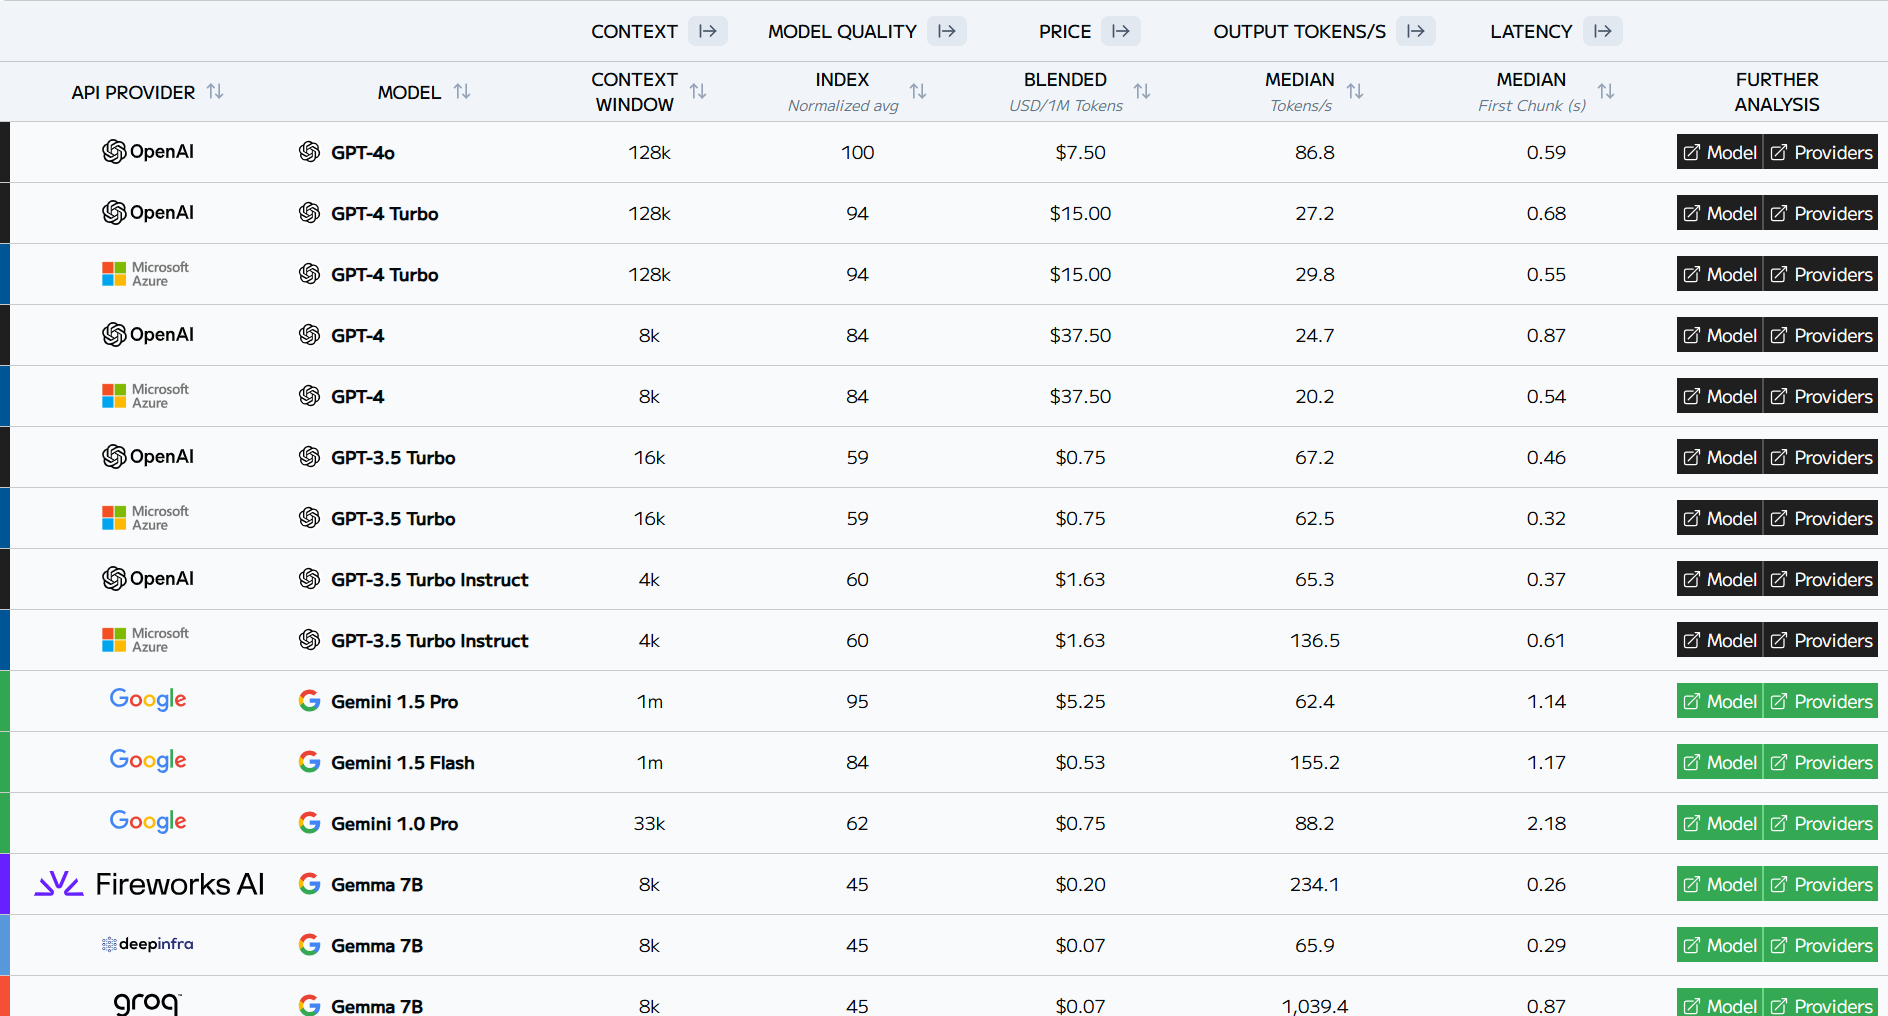
\includegraphics[width=\linewidth]{./figures/LLM-Perf-P1.png}
    \end{subfigure}
    \begin{subfigure}{.97\textwidth}
        \centering
        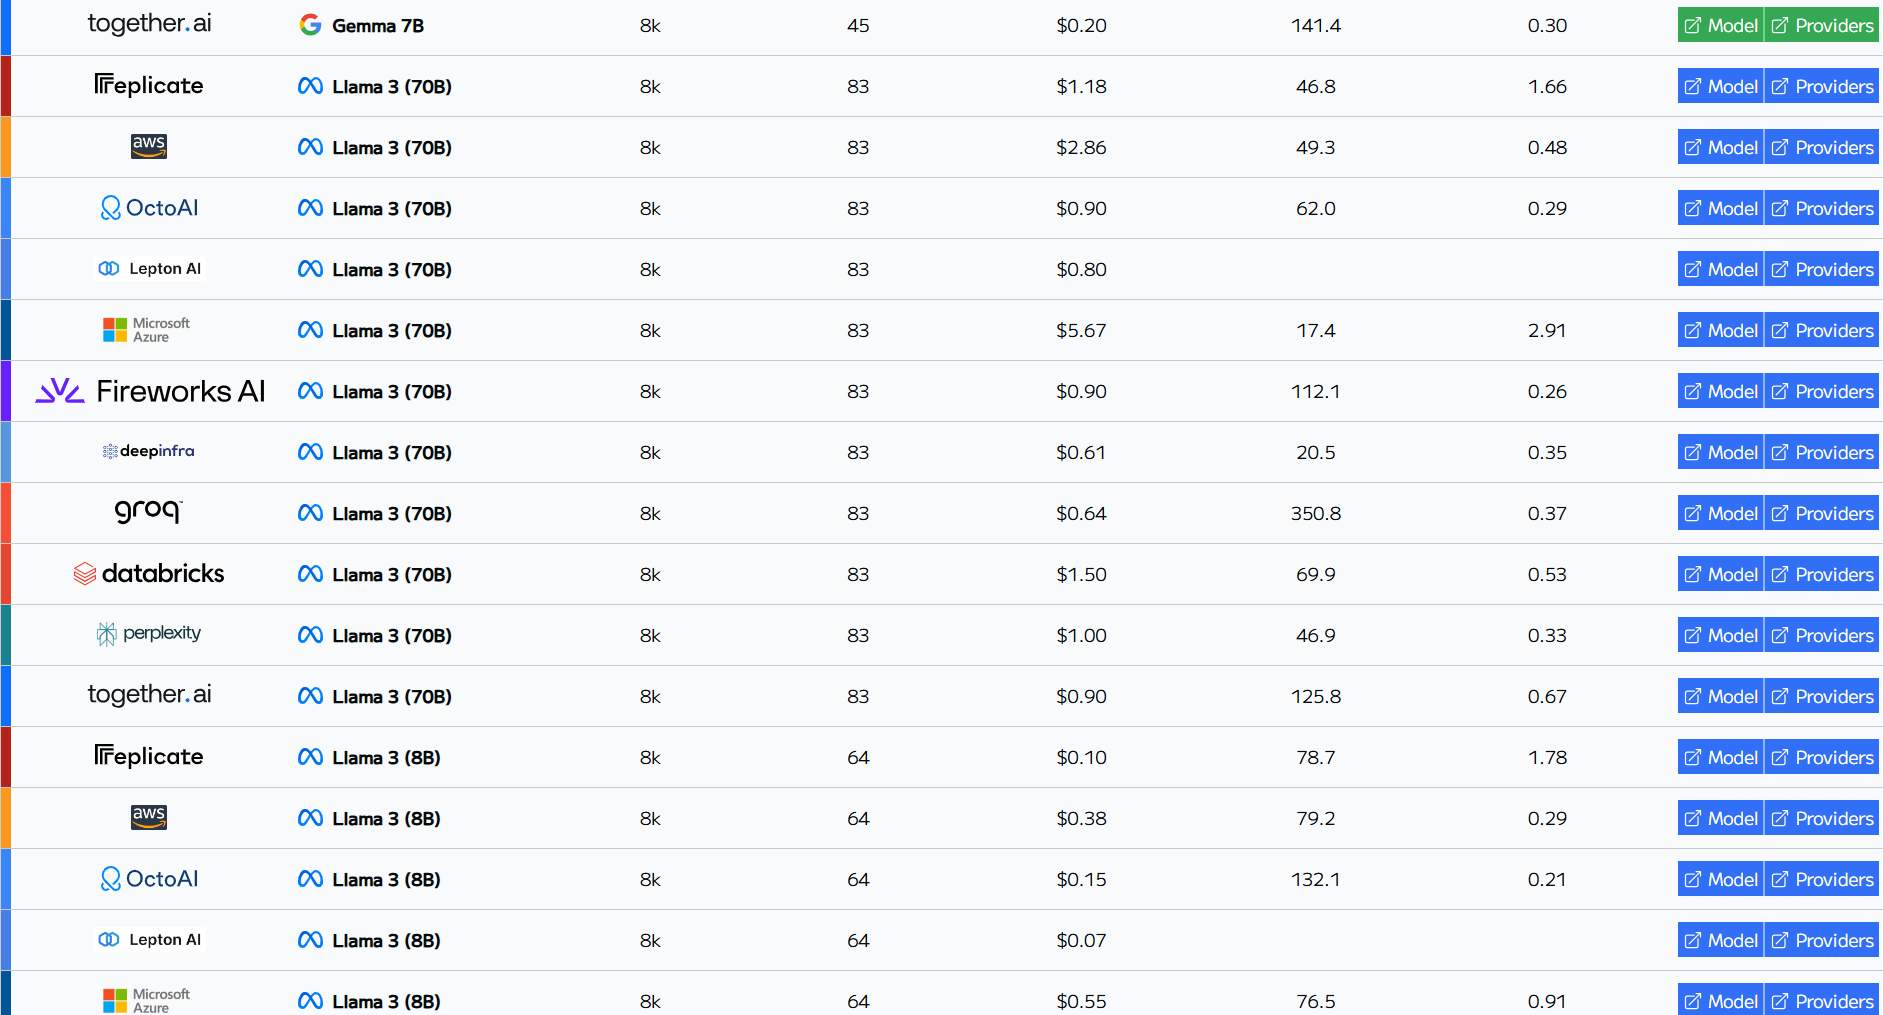
\includegraphics[width=\linewidth]{./figures/LLM-Perf-P2.png}
    \end{subfigure}
    \caption{API Providers and LLM Performance Leaderboard \href{https://huggingface.co/spaces/ArtificialAnalysis/LLM-Performance-Leaderboard}{[ArtificialAnalysis/LLM-Performance-Leaderboard space on Hugging Face]}}.
\end{figure}
\newpage

\subsection{Entreprise Knowledge Base Augmentation}
The main issue with Large Language Models is that they are confined to the data they were trained on. This means they do not have access to information about recent events or private EKB, thus the need to implement methods to allow the continuous upload of documents into the vector store.\newline
In our case, there is no need to collect data as this project does not involve training or fine-tuning models, but rather providing methods that allow scraping and uploading information from various sources.\newline
For this purpose, an anticipatory study of the system's knowledge augmentation methods have resulted in identifying the following requirements :
\begin{itemize}
    \item Offline files: Support for the different offline document formats (text files, pdfs, word documents, powerpoint presentations, e-book format/epub, markdown documentation)
    \item Web Scraping: A single web page from a URL, or recursively scraping its child pages
    \item Search Engine Results: By using some of Search Engine APIs, connect the user's query directly to search results and then scrape information for the returned URLs.
    \item AI-generated researches: LLMs can also automatize the traditional process of searching the web, reading webpages, and artificially generating a report based on those analyzed pages.
\end{itemize}